
\appendix

\section{Függelék}
\label{sec:sip_message_xml_fuggelek}

\subsection{SIP MESSAGE kérés törzsében átvitt XML tartalom sémája}

\fontsize{10}{10}
\begin{verbatim}
<?xml version="1.0" encoding="UTF-8"?>
<xs:schema xmlns:xs="http://www.w3.org/2001/XMLSchema">

    <!-- InfoMessage -->
    <xs:element name="infoMessage">
        <xs:complexType>
            <xs:sequence>              
                <xs:element name="info_type">
                    <xs:simpleType>
                        <xs:restriction base="xs:string">
                            <xs:enumeration value="NOTIFY_USER"/>
                            <xs:enumeration value="MESSAGE_DATA"/>
                            <xs:enumeration value="DOWNLOAD_CONTENT"/>
                            <xs:enumeration value="DELETE_MESSAGE"/>
                        </xs:restriction>
                    </xs:simpleType>
                </xs:element>
                <xs:element name="detailList">
                    <xs:complexType>
                        <xs:sequence>
                            <xs:element name="detail" 
                                        type="InfoDetail" 
                                        maxOccurs="unbounded"/>
                        </xs:sequence>
                    </xs:complexType>
                </xs:element>
            </xs:sequence>
        </xs:complexType>
    </xs:element>

    <xs:complexType name="InfoDetail">
        <xs:sequence>
            <xs:element name="sender" type="userInfo" minOccurs="0"/>      
            <xs:element name="id" type="xs:string"/>
            <xs:element name="content" type="contentDescription" 
                                       minOccurs="0"/>
            <xs:element name="subject" type="xs:string" minOccurs="0"/>
            <xs:element name="sent_at" type="xs:dateTime" minOccurs="0"/>
            <xs:element name="recipientList" minOccurs="0">
                <xs:complexType>
                    <xs:sequence>
                        <xs:element name="recipient" type="userInfo" 
                                    maxOccurs="unbounded"/>
                    </xs:sequence>
                </xs:complexType>
            </xs:element>
        </xs:sequence>
    </xs:complexType>
    
    <xs:element name="messageInfoContainer">
        <xs:complexType>
            <xs:sequence>
                <xs:element name="sender" type="userInfo"/>                
                <xs:element name="id" type="xs:string"/>
                <xs:element name="subject" type="xs:string"/>
                <xs:element name="sent_at" type="xs:dateTime"/>
                <xs:element name="status" type="xs:string"/>
                <xs:element name="contentDescription" 
                            type="contentDescription"/>
            </xs:sequence>
        </xs:complexType>
    </xs:element>
    
    <xs:complexType name="contentDescription">
            <xs:sequence>
                <xs:element name="mimeType">
                    <xs:simpleType>
                        <xs:restriction base="xs:string">
                            <xs:enumeration value="image/jpeg"/>                                       
                            <xs:enumeration value="image/bmp"/>
                            <xs:enumeration value="image/gif"/>
                            <xs:enumeration value="image/png"/>                                     
                            <xs:enumeration value="audio/mpeg"/>
                            <xs:enumeration value="audio/x-wav"/>                               
                            <xs:enumeration value="video/x-msvideo"/>
                            <xs:enumeration value="video/mpeg"/>
                        </xs:restriction>
                    </xs:simpleType>
                </xs:element>
                <xs:element name="size" type="xs:int" minOccurs="0"/>
                <xs:element name="content_available" 
                            type="xs:boolean" minOccurs="0"/>
            </xs:sequence>        
    </xs:complexType>
    
    <xs:complexType name="userInfo">
        <xs:sequence>
            <xs:element name="name" type="xs:string"/>
            <xs:element name="sip_uri" type="xs:string"/>
        </xs:sequence>
    </xs:complexType>

</xs:schema>
\end{verbatim}
\fontsize{12}{12} 

\newpage 
\subsection{Példák a MESSAGE kérés törzsében található XML-ekre}

\subsubsection*{Multimédia üzenet címzettjeit, egyéb adatait tartalmazó üzenet esetén}
\fontsize{10}{10}
\begin{verbatim}
<?xml version="1.0" encoding="UTF-8" standalone="yes"?>
   <infoMessage>
      <info_type>MESSAGE_DATA</info_type>
      <detailList>
         <detail>
            <sender>
               <name>Alice</name>
               <sip_uri>sip:alice@ericsson.com</sip_uri>
            </sender>
            <id>a190c0316393435</id>
            <content>
               <mimeType>audio/mpeg</mimeType>
               <size>85726</size>
            </content>
            <subject>Message subject field</subject>
            <recipientList>
               <recipient>
                  <name>Bob</name>
                  <sip_uri>sip:bob@ericsson.com</sip_uri>
               </recipient>
               <recipient>
                  <name>Coco</name>
                  <sip_uri>sip:coco@ericsson.com</sip_uri>
               </recipient>
            </recipientList>
         </detail>
      </detailList>
   </infoMessage>
\end{verbatim}
\fontsize{12}{12} 

\subsubsection*{Értesítő üzenet esetén}
\fontsize{10}{10}
\begin{verbatim}
<?xml version="1.0" encoding="UTF-8" standalone="yes"?>
   <infoMessage>
      <info_type>NOTIFY_USER</info_type>
      <detailList>
         <detail>
            <sender>
               <name>Alice</name>
               <sip_uri>sip:alice@ericsson.com</sip_uri>
            </sender>
            <id>b807dc87433043d</id>
            <content>
               <mimeType>audio/mpeg</mimeType>
               <size>85726</size>
            </content>
            <subject>Subject</subject>
            <sent_at>2011-05-01T18:27:50.000+02:00</sent_at>
         </detail>
      </detailList>
   </infoMessage>
\end{verbatim}
\fontsize{12}{12} 

\subsubsection*{Adott multimédia tartalom letöltési igény esetén}
\fontsize{10}{10}
\begin{verbatim}
<?xml version="1.0" encoding="UTF-8" standalone="yes"?>
   <infoMessage>
      <info_type>DOWNLOAD_CONTENT</info_type>
      <detailList>
         <detail>
            <id>b807dc87433043d</id>
         </detail>
      </detailList>
   </infoMessage>
\end{verbatim}
\fontsize{12}{12} 

\subsubsection*{Multimédia üzenetek megtekintés nélküli törlését jelző kérés esetén}
\fontsize{10}{10}
\begin{verbatim}
<?xml version="1.0" encoding="UTF-8" standalone="yes"?>
   <infoMessage>
      <info_type>DELETE_MESSAGE</info_type>
      <detailList>
         <detail>
            <id>b807dc87433043d</id>
         </detail>
         <detail>
            <id>a190c0316393435</id>
         </detail>
      </detailList>
   </infoMessage>
\end{verbatim}
\fontsize{12}{12} 
\newpage 

\section{Függelék}
\label{sec:sql_utasitasok_fuggelek}

\noindent
{\bf Az adatbázis táblákat létrehozó SQL utasítások}

\fontsize{10}{10}
\begin{verbatim}
CREATE TABLE MESSAGES
(
  ID INT NOT NULL AUTO_INCREMENT,
  MESSAGE_ID VARCHAR(200) NOT NULL,
  CONTENT BLOB
  SENDER_NAME VARCHAR(150)
  SENDER_SIP_URI VARCHAR(150)
  SENT_AT DATE
  SUBJECT VARCHAR(250)
  CONTENT_TYPE VARCHAR(50),
  CONTENT_SIZE INT
  CONSTRAINT pk_messages PRIMARY KEY(ID),
  CONSTRAINT uq_msrp_message_id UNIQUE(MESSAGE_ID)
) ENGINE=InnoDB DEFAULT CHARSET=utf8;
\end{verbatim}
\fontsize{12}{12}

\fontsize{10}{10}
\begin{verbatim}
CREATE TABLE RECIPIENTS
(
  ID INT NOT NULL AUTO_INCREMENT,
  MESSAGE_ID INT NOT NULL,
  NAME VARCHAR(150)
  SIP_URI VARCHAR(150)
  DELIVERY_STATUS VARCHAR(30)
  CONSTRAINT pk_recipients PRIMARY KEY (ID)
  CONSTRAINT fk_messages FOREIGN KEY (MESSAGE_ID) REFERENCES MESSAGES(ID)
) ENGINE=InnoDB DEFAULT CHARSET=utf8;
\end{verbatim}
\fontsize{12}{12}

\newpage

\section{Függelék}
\label{sec:kliens_screenshots}

\noindent
{\bf A kliens alkalmazás főablaka (\ref{fig:screenshot02}.~ábra)}

\begin{figure}[htb]
\center
\resizebox{5cm}{!}{
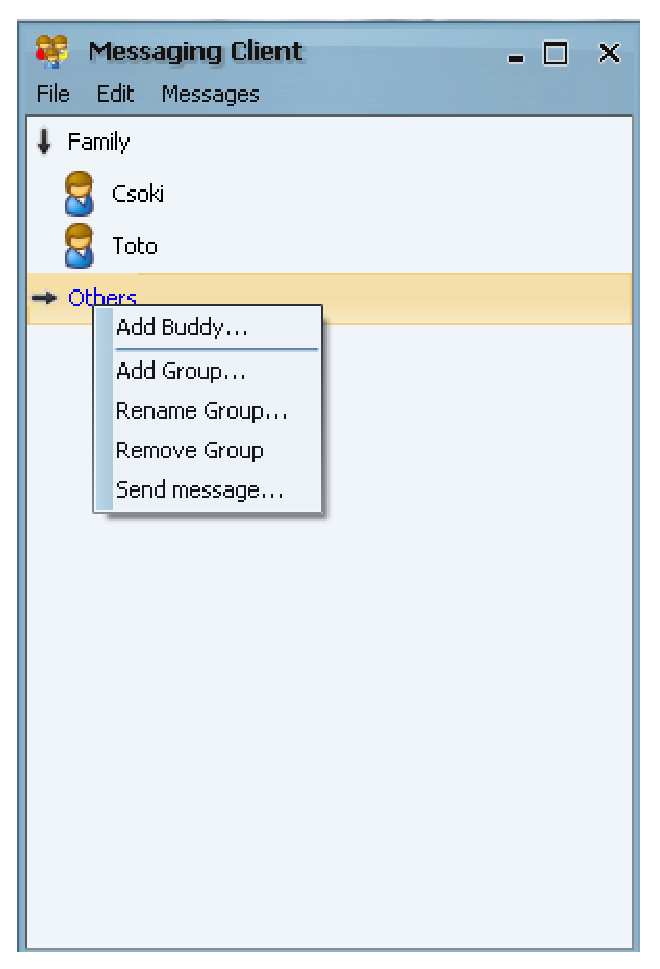
\includegraphics{img/screenshot02.eps}}
\caption{Az induló képernyő}
\label{fig:screenshot_main}
\end{figure}

\noindent
{\bf Egyéb ablakok (\ref{fig:screenshot3}.~ábra)}


\begin{figure}[htbp]
  \begin{center}
    \subfloat[Új üzenet létrehozása]{\label{fig:screenshot03_1}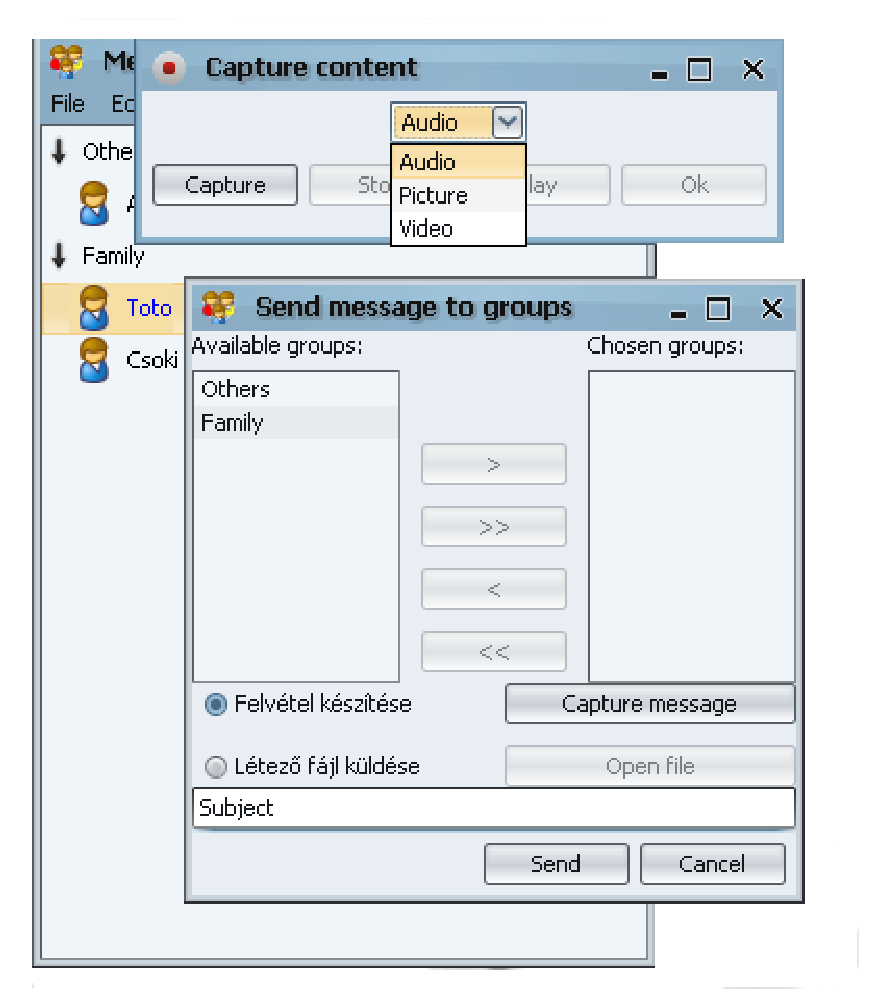
\includegraphics[scale=0.45]{img/screenshot03.eps}}
    \hspace{0.1in}
    \subfloat[Az elküldött és beérkező üzenetek]{\label{fig:screenshot03_2}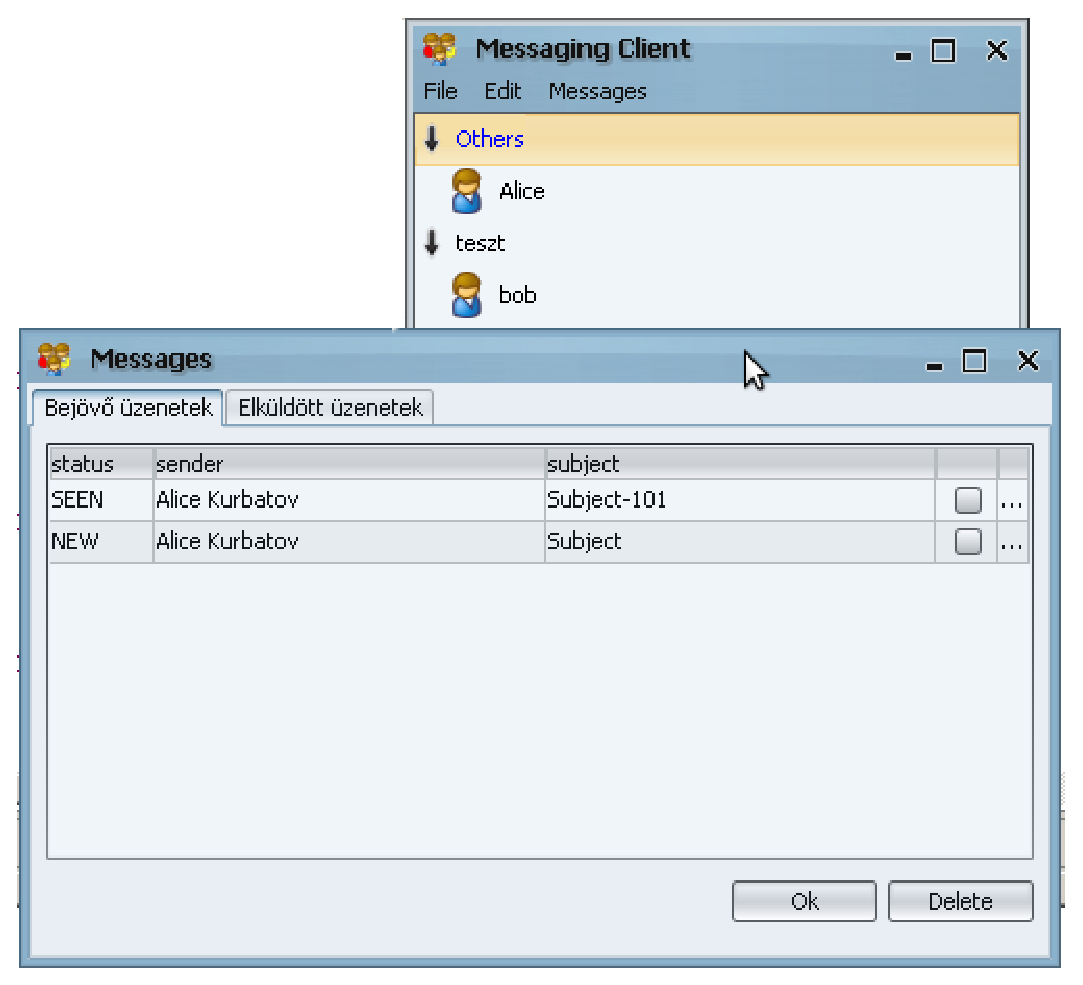
\includegraphics[scale=0.45]{img/screenshot01.eps}}
  \end{center}
  \caption{Új multimédia üzenet létrehozás, illetve a levelesláda megtekintés}
  \label{fig:screenshot3}
\end{figure}

